\documentclass[a4paper,UKenglish,cleveref, autoref, thm-restate]{lipics-v2021}
%This is a template for producing LIPIcs articles. 
%See lipics-v2021-authors-guidelines.pdf for further information.
%for A4 paper format use option "a4paper", for US-letter use option "letterpaper"
%for british hyphenation rules use option "UKenglish", for american hyphenation rules use option "USenglish"
%for section-numbered lemmas etc., use "numberwithinsect"
%for enabling cleveref support, use "cleveref"
%for enabling autoref support, use "autoref"
%for anonymousing the authors (e.g. for double-blind review), add "anonymous"
%for enabling thm-restate support, use "thm-restate"
%for enabling a two-column layout for the author/affilation part (only applicable for > 6 authors), use "authorcolumns"
%for producing a PDF according the PDF/A standard, add "pdfa"

%\pdfoutput=1 %uncomment to ensure pdflatex processing (mandatatory e.g. to submit to arXiv)
%\hideLIPIcs  %uncomment to remove references to LIPIcs series (logo, DOI, ...), e.g. when preparing a pre-final version to be uploaded to arXiv or another public repository

%\graphicspath{{./graphics/}}%helpful if your graphic files are in another directory


\usepackage{amsmath}
\usepackage{cite}
%\let\proof\relax
%\let\endproof\relax

\sloppy


\usepackage{cleveref}
\usepackage{amsthm}
\usepackage{amssymb}
\usepackage{amsfonts}
\usepackage{mathrsfs}
\usepackage{wrapfig} %wrap the text around the picture


\usepackage{thmtools} 
\usepackage{thm-restate}

\usepackage{caption} %for subfigure - join multiple figures and add captions
\usepackage{subcaption}
\usepackage{changepage} %inside figure we can put \begin{adjustwidth}{-1cm}{-1cm} \end{adjustwidth} and we can ignore the margins
\usepackage{mathtools} % write text [under]{over} arrow $\xrightarrow[\text{world}]{\text{hello}}$

\usepackage{graphicx}
\graphicspath{{Figures/}}

\usepackage{tikz}

\usetikzlibrary{arrows,decorations.pathmorphing,decorations.pathreplacing,backgrounds,positioning,fit,matrix}
\usetikzlibrary{shapes,calc,patterns,arrows.meta}
\tikzset{
	vert/.style={circle,inner sep=1.5,fill=white,draw=black,minimum size=.3cm},
    dummy/.style={circle,fill=black,draw=black,inner sep=2.5},
	edge/.style={color=black, thick},
	diredge/.style={->,>={Stealth[width=8pt,length=8pt]},color=black, thick},
	timelabel/.style={fill=white,font=\footnotesize, text centered},
	wave/.style={decorate,decoration={coil,aspect=0}},
	dirwave/.style={->, >={Stealth[width=8pt,length=8pt]},decorate,decoration={coil,aspect=0}},
	diredge2/.style={->,>={Stealth[width=8pt,length=8pt]}}
}

%\usepackage{enumitem} %enumerate 
\usepackage{enumerate}
\usepackage{todonotes}
\newcommand{\todonkl}[2][]{\todo[color=red!100!green!33,#1]{NKL:\\ #2}} %todo note that starts with NKL:
\setlength{\marginparwidth}{3.7cm} %setting the length of todonote


\usepackage{comment}

\usepackage{algorithm}
\usepackage[noend]{algpseudocode}


%font encoding
\usepackage[T1]{fontenc}
\usepackage[utf8]{inputenc}
\usepackage{lmodern}

\usepackage{hyperref}

\crefname{claim}{Claim}{Claims}

%\usepackage{natbib}

\newcommand{\ie}{i.\,e.,\ }
\renewcommand{\st}{s.\,t.,\ }
\newcommand{\NP}{\textrm{NP}}
\newcommand{\APX}{\textrm{APX}}
\newcommand{\FPT}{\textrm{FPT}}
\newcommand{\XP}{\textrm{XP}}

\newcommand{\NN}{\mathbb{N}}
\newcommand{\ZZ}{\mathbb{Z}}
\newcommand{\RR}{\mathbb{R}}
\newcommand{\QQ}{\mathbb{Q}}


%%%%%%%%%%%%%%%%%%%%%%%%%%%%%%%% Defining a problem
%%%%%%%%%%%%%%%%%%\problemdef{NAME} {Input} {Output}
\usepackage{tabularx}
\newcommand{\problemdef}[3]{
	\begin{center}
		\begin{minipage}{0.95\textwidth}
			\noindent
			#1
			\vspace{5pt}\\
			\setlength{\tabcolsep}{3pt}
			\begin{tabularx}{\textwidth}{@{}lX@{}}
				\textbf{Input:}& #2 \\
				\textbf{Question:}& #3
			\end{tabularx}
		\end{minipage}
	\end{center}
}


%%%%%%%%%%%%%%%%%%%%%%%%%%%%%%%%%% PROBLEMS NAMES
%% One label per edge, period Delta, exact realization
\newcommand{\deltaExactLong}{\textsc{Simple periodic Temporal Graph Realization}}
\newcommand{\deltaExact}{\textsc{Simple TGR}}

\newcommand{\deltaSymExactLong}{\textsc{Simple symmetric periodic Temporal Graph Realization}}
\newcommand{\deltaSymExact}{\textsc{Simple Symmetric TGR}}

%% k labels per edge, period Delta, exact realization
\newcommand{\kDeltaExactLong}{\textsc{$(k,\Delta)$-periodic Exact Temporal Graph Realization}}
\newcommand{\kDeltaExact}{\textsc{$(k,\Delta)$-TGR}}

%% One label per edge, period Delta, upper-bounded realization
\newcommand{\DeltaUpperBoundLong}{\textsc{Simple $\Delta$-periodic Upper-Bounded Temporal Graph Realization}}
\newcommand{\deltaUpperBound}{\textsc{Simple Upper-Bounded TGR}}

%% k labels per edge, period Delta, lower-bound realization
\newcommand{\kDeltaLowerBoundLong}{\textsc{Simple $\Delta$-periodic Lower-Bounded Temporal Graph Realization}}


\bibliographystyle{plainurl}% the mandatory bibstyle

\title{Realizing temporal graphs from fastest paths II} %TODO Please add

%\titlerunning{Dummy short title} %TODO optional, please use if title is longer than one line

\author{Nina Klobas}{Department of Computer Science, Durham University, UK}{nina.klobas@durham.ac.uk}{ https://orcid.org/0000-0002-8024-5782}{}

\author{George B. Mertzios}{Department of Computer Science, Durham University, UK}{george.mertzios@durham.ac.uk}{https://orcid.org/0000-0001-7182-585X}{Supported by the EPSRC grant EP/P020372/1.}

\author{Hendrik~Molter}{Department of Computer Science, Ben-Gurion~University~of~the~Negev, 
	Beer-Sheva, 
	Israel}{molterh@post.bgu.ac.il}{https://orcid.org/0000-0002-4590-798X}{Supported by the ISF, grant No.~1456/18, and the ERC, grant number 949707.}

\author{Paul G. Spirakis}{Department of Computer Science, University of Liverpool, UK}{p.spirakis@liverpool.ac.uk}{https://orcid.org/0000-0001-5396-3749}{Supported by the EPSRC grant EP/P02002X/1.}

\authorrunning{Nina Klobas, George B. Mertzios, Hendrik Molter, and Paul G. Spirakis} %TODO mandatory. First: Use abbreviated first/middle names. Second (only in severe cases): Use first author plus 'et al.'

\Copyright{Nina Klobas, George B. Mertzios, Hendrik Molter, and Paul G. Spirakis} %TODO mandatory, please use full first names. LIPIcs license is "CC-BY";  http://creativecommons.org/licenses/by/3.0/

\ccsdesc[500]{Theory of computation~Graph algorithms analysis}
\ccsdesc[500]{Mathematics of computing~Discrete mathematics}
%TODO mandatory: Please choose ACM 2012 classifications from https://dl.acm.org/ccs/ccs_flat.cfm 

\keywords{Temporal graph, periodic temporal labeling, fastest temporal path, graph realization, temporal connectivity.} %TODO mandatory; please add comma-separated list of keywords

\category{} %optional, e.g. invited paper

\relatedversion{} %optional, e.g. full version hosted on arXiv, HAL, or other respository/website
%\relatedversiondetails[linktext={opt. text shown instead of the URL}, cite=DBLP:books/mk/GrayR93]{Classification (e.g. Full Version, Extended Version, Previous Version}{URL to related version} %linktext and cite are optional

%\supplement{}%optional, e.g. related research data, source code, ... hosted on a repository like zenodo, figshare, GitHub, ...
%\supplementdetails[linktext={opt. text shown instead of the URL}, cite=DBLP:books/mk/GrayR93, subcategory={Description, Subcategory}, swhid={Software Heritage Identifier}]{General Classification (e.g. Software, Dataset, Model, ...)}{URL to related version} %linktext, cite, and subcategory are optional

%\funding{(Optional) general funding statement \dots}%optional, to capture a funding statement, which applies to all authors. Please enter author specific funding statements as fifth argument of the \author macro.

%\acknowledgements{I want to thank \dots}%optional

%\nolinenumbers %uncomment to disable line numbering



%Editor-only macros:: begin (do not touch as author)%%%%%%%%%%%%%%%%%%%%%%%%%%%%%%%%%%
\EventEditors{John Q. Open and Joan R. Access}
\EventNoEds{2}
\EventLongTitle{42nd Conference on Very Important Topics (CVIT 2016)}
\EventShortTitle{CVIT 2016}
\EventAcronym{CVIT}
\EventYear{2016}
\EventDate{December 24--27, 2016}
\EventLocation{Little Whinging, United Kingdom}
\EventLogo{}
\SeriesVolume{42}
\ArticleNo{23}
%%%%%%%%%%%%%%%%%%%%%%%%%%%%%%%%%%%%%%%%%%%%%%%%%%%%%%

\begin{document}
	\maketitle
	
\problemdef{\deltaSymExactLong\ (\deltaSymExact)}
{An $n \times n$ symmetric matrix $D$, a positive integer $\Delta$.}
{Does there exist a graph $G=(V,E)$ with vertices $\{v_1,\ldots,v_{n}\}$ 
	and a $\Delta$-periodic labeling $\lambda: E \rightarrow \{1,2,\ldots,\Delta\}$ such that, 
	for every $i,j$, the duration of the fastest temporal path from $v_i$ to $v_j$ in the $\Delta$-periodic temporal graph $(G,\lambda,\Delta)$ is $D_{i,j}$?}
	
\problemdef{\DeltaUpperBoundLong (\deltaUpperBound)}
{A static graph $G=(V,E)$ with $n$ vertices, $n \times n$ matrix $D$ of positive integers and a bijective mapping $\phi$ from vertices $V$ of $G$ to the rows/columns of the matrix $D$.}
{Does there exist a $\Delta$-periodic labeling $\lambda: E \rightarrow \{1,2,\ldots,\Delta\}$ such that, 
	for every $i,j$, the duration of the fastest temporal path from $v_i$ to $v_j$ in the $\Delta$-periodic temporal graph $(G,\lambda,\Delta)$ is \emph{at most} $D_{\phi(i),\phi(j)}$.}

\section{Preliminaries and notation}
\todo[inline]{This section is copied from our paper}

An interval in $\mathbb N$ from $a$ to $b$ is denoted by $[a,b] = \{ i\in \mathbb N  :  a \leq i \leq b\}$; similarly, $[a] = [1,a]$.
An undirected graph~$G=(V,E)$ consists of a set~$V$ of vertices 
and a set~$E \subseteq V \times V$ of edges.
For a graph~$G$, we also denote by~$V(G)$ and~$E(G)$ the vertex and edge set of~$G$, respectively.
We denote an edge $e \in E$ between vertices $u,v \in V$ as a set $e=\{u,v\}$.
For the sake of simplicity of the representation, an edge $e$ is sometimes also denoted by $uv$. 
A path~$P$ in $G$ is a subgraph of $G$ with vertex set~$V(P)=\{v_1,\dots,v_k\}$ and edge set~$E(P)=\{\{v_i,v_{i+1}\} :  1\leq i<k\}$
(we often represent path~$P$ by the tuple~$(v_1,v_2,\dots,v_k)$).

Let $v_1,v_2,\ldots,v_n$ be the $n$ vertices of the graph $G$. 
For simplicity of the presentation~--and with a slight abuse of notation--~we refer during the paper to the entry $D_{i,j}$ of the matrix $D$ as 
$D_{a,b}$, where $a=v_i$ and $b=v_j$. That is, we put as indices of the matrix $D$ the corresponding vertices of $G$ whenever it is clear from the context.

We denote with $d(u,v,P)$ the duration of the fastest temporal path from $u$ to $v$ along path $P$. Note that $d(u,v,P) \geq d(u,v)$.

We remark that a fastest path between two vertices in a temporal graph can be computed in polynomial time~\cite{xuan_computing_2003,Wu2016Efficient}.
Hence, given a $\Delta$-periodic temporal graph $(G,\lambda,\Delta)$, we can compute in polynomial-time  the matrix $D$
which consists of durations of fastest temporal paths among all pairs of vertices in $(G,\lambda,\Delta)$.


\begin{definition}[Travel delays] \label{def:travelDelays}
	Let $(G, \lambda)$ be a $\Delta$-periodic temporal graph.
	Let $e_1=uv$ and $e_2=vz$ be two incident edges in $G$ with $e_1 \cap e_2 = v$.
	We define the \emph{travel delay} from $u$ to $z$ at vertex $v$, denoted with $\tau_v^{uz}$,
	as the difference of the labels of $e_2$ and $e_1$, where we subtract the value of the label of $e_1$ from the label of $e_2$,  modulo~$\Delta$.
	More specifically:
	\begin{equation}\label{eq:def-VertexWaitingTime}
		\tau_v^{uz} \equiv \lambda (e_2) - \lambda(e_1) \pmod \Delta.
	\end{equation}
	Similarly, $\tau_v^{zu} \equiv \lambda (e_1) - \lambda(e_2) \pmod \Delta$.
\end{definition}
Intuitively, the value of $\tau_v^{uz}$ represents how long a temporal path waits at vertex $v$ when first taking edge $e_1=uv$ and then edge $e_2 = vz$.





\section{D is symmetric}
Before studying the problem in general let us first focus on two restricted cases.
\begin{theorem}
	If the input graph $G$ of \deltaSymExact\ is a clique or a $C_4$ then the problem is polynomial-time solvable. 
\end{theorem}

\begin{proof}
	We split the proof in two cases.
	
	First, when the input graph is a clique. In this case the desired labeling $\lambda$ can be arbitrary (i.e. $\lambda(e) \in [\Delta]$ for all $e \in E$), 
	as all vertices are on distance (and duration) $1$ from each other.
	Therefore 
	\begin{equation*}
		D_{i,j} =
		\begin{cases}
			0 & \text{if $i = j$}, \\
			1 & \text{else}
		\end{cases},
	\end{equation*}
	which is a symmetric matrix.
	
	Second, when the input graph $G$ is a $C_4$. Let $v_1, v_2, v_3, v_4$ be the vertices of $G$ with edges $e_1 = v_1 v_2, e_2 = v_2 v_3, e_3 = v_3 v_4, e_4 = v_4 v_1$.
	Now we set $\lambda(e_1) = \lambda (e_3) = \alpha$ and $\lambda(e_2) = \lambda(e_4) = \beta$, where w.l.o.g. $\alpha > \beta$.
	Let $\gamma = min \{ \alpha - \beta, \Delta + \beta - \alpha\}$,
	i.e. $\gamma$ is the minimum travel delay at vertex $v_i$ when traversing first the edge $e_{i-1}$ and then $e_i$ (indices are taken modulo $4$).
	We get that 
	\begin{equation*}
		D_{i,j} =
		\begin{cases}
			0 & \text{if $i = j$}, \\
			1 & \text{if $v_i$ and $v_j$ are neighbors},\\
			\gamma + 1 & \text{else}\\
		\end{cases}
	\end{equation*}
	Note, if $\alpha = \beta$ then the values in $D$ of non-neighboring vertices (i.e. vertices on distance $2$ from each other)
	are exactly $\Delta + 1$.
\end{proof}


Observe the following.
\begin{claim}
	Let $P = (u, v, w)$ be a path of length $2$, and let $(P,\lambda)$ be a $\Delta$-periodic temporal graph,
	 then $D_{u,w} = D_{w,v}$ iff $\tau_v^{uw} = \tau_v^{wu}$. 
\end{claim}
\begin{proof}
	Let us denote with $\alpha = \lambda(uv)$ and  $\beta = \lambda(vw)$,
	w.l.o.g. we suppose also that $\alpha > \beta$.
	Then $d(u,w) = \Delta + \beta - \alpha + 1$ 
	and $d(w,u) = \alpha - \beta + 1$.
	By the definition of travel delays we get $d(u,w) = \tau_v^{uw} + 1$ and $d(w,u) = \tau_v^{wu} + 1$. 
	Since $D_{u,w} = D_{w,v}$ we get that $\tau_v^{uw} = \tau_v^{wu}$.
\end{proof}

From the above claim we get the following.

\begin{claim}
	Let $P = (u, v, w)$ be a path of length $2$, and let $(P,\lambda)$ be a $\Delta$-periodic temporal graph, 
	then $D_{u,w} = D_{w,v}$
	if and only if
    for every edge $e \in E(P)$ it holds that that
	$\lambda(e) \in \{\frac{\Delta}{2}, \Delta\}$, when $\Delta$ is even and
	$\lambda(e) = \Delta$, when $\Delta$ is odd.
\end{claim}

\begin{proof}
		Let us denote with $\alpha = \lambda(uv)$ and  $\beta = \lambda(vw)$,
		w.l.o.g. we suppose also that $\alpha > \beta$.
		Since
		$\tau_v^{uw} = \tau_v^{wu}$
		we get that
		\begin{equation*}
			\Delta + \beta - \alpha \equiv \alpha - \beta \pmod\Delta,
		\end{equation*}
		which is equivalent to
		\begin{equation}\label{eq:sol-delta}
			\Delta  \equiv 2 (\alpha - \beta) \pmod\Delta.
		\end{equation}
		Since $\alpha > \beta$, the only possible solution of \cref{eq:sol-delta} is when $\beta \equiv \frac{\alpha}{2} \pmod \Delta$, which exists only in the case when $\Delta$ is even.
		If we now allow $\alpha = \beta$ then we get another solution of \cref{eq:sol-delta}.
		
		W.l.o.g. we can now suppose that $\alpha = \Delta$.
		If $\Delta$ is odd, we have a unique solution with the value $\alpha=\beta = \Delta$,
		while in the case when $\Delta$ is even we get that $\alpha, \beta \in \{\Delta, \frac{\Delta}{2}\}$. 
\end{proof}

In the case of a general graph $G$, the above still has to hold for any two vertices on distance $2$ apart.
Therefore we get the following two results.

\begin{claim}\label{claim:symmetric-odd}
	When $\Delta$ is odd, the only possibility of the matrix $D$, of all durations, being symmetric is when all labels of $G$ are the same.
\end{claim}

\begin{claim}\label{claim:symmetric-even}
	When $\Delta$ is even, the only possibility of the matrix $D$, of all durations, being symmetric is when all labels of $G$ are from $\{\frac{\Delta}{2}, \Delta\}$.
\end{claim}

From all of the above we get the following result.
\begin{theorem}
	\deltaSymExact\ can be solved in polynomial time.
\end{theorem}
\todo[inline]{Not all edges need to have labels from $\{\Delta, \Delta/2 \}$ - some of them can have whatever label. Think how these edges/graphs look like (example ``diamond with an inner path of length 2'' aka, $C_4$ with an extra vertex in the middle connecting a pair of opposite vertices).}
\begin{proof}
	TODO
\end{proof}

\section{Upper bounds in the matrix D}

\subsection{\deltaUpperBound\ on paths}
We start by investigating the complexity of the problem \DeltaUpperBoundLong\ in the case when the underlying graph of the input instance is a path.

\begin{comment}
Let $(G,D)$ be an instance of \deltaUpperBound\, where $G$ is a path of length $n$.
Denote with $v_0,v_1, v_2, \dots, v_n$ the vertices of $G$ where $v_{i}v_{i+1} \in E(G)$, for all $i \in [n]$.
And let $\lambda$ be a labelling that we are trying to construct (\ie a labeling satisfying conditions of the problem).
The following must hold.
\begin{enumerate}[(a)]
	\item \label{path:enum-1}
 Let $i,j,k \in [n]$, where $i < k < j$, and let $D_{i,j} \leq D_{i,k}$. 
 Then the temporal path $P_{i,k}$ from $v_i$ to $v_k$ cannot be of duration more than $D_{i,j} - (k-j)$,
 which implies that $D_{i,k} \leq D_{i,j} - (k-j)$.
 
 This holds because $P_{i,k}$ is a subpath of the temporal path $P_{i,j}$ from $v_i$ to $v_j$,
 therefore we can brake down $P_{i,j}$ into two parts, $P_{i,k}$ and the path $P_{k,j}$ from $v_k$ to $v_j$.
 Since $P_{k,j}$ consists of $k-j$ edges we need at least $k-j$ time to traverse it, so the duration of $P_{i,k}$ cannot take more than $D_{i,j} - (k-j)$ time.

    \item \label{path:enum-2}
     For any two vertices $v_i, v_{i+2}$ on distance two apart the following holds $d(i, i+2) + d(i+2, i) = \Delta + 2$.
     Therefore $D_{i,i+2} + D_{i+2,i} \geq \Delta + 2$.
     We can generalize this observation for any two vertices on distance $k$ apart and get 
     $D_{i,i+k} + D_{i+k,i} \geq (k-1) \Delta + 2$.

    %    \item \label{path:enum-3}
    %    From the definition of temporal paths, it follows that $d(i,j) = d(i,k) + d(k-1, j) - 1$, where $i,j \in [n]$, with $i<j$ and $k \in [i+1,j-1]$.
    %    Therefore $D_{i,j} \leq D_{i,k} + D_{k-1,j} -1$.
\end{enumerate}

From all of the above properties we create a polynomial-time algorithm that transforms the input matrix $D$ into a reduced one, without affecting any potential solutions.
The algorithm performs the following steps.
\begin{enumerate}
    \item A vertex $v_i$ is on the distance $0$ from itself, and at distance $1$ from its neighbors,
    which means it is also on the duration $0$ and $1$ from them, respectively.
    Therefore we set all the diagonal values of $D$ to $0$, and the upper and lower diagonals to $1$.
    \item 
    From the property~(\ref{path:enum-1}) it follows that the values in every row $i$ the values have to be strictly increasing (resp.~decreasing) from $D_{i,i}$ to $D_{i,n}$ (resp.~$D_{i,1}$).
    Therefore we loop through each row of $D$ and whenever we encounter 
    a row that does not obey this rule, we use the property~(\ref{path:enum-1}) to modify its entries.
\end{enumerate}
For the matrix $D$ we can also check that the property~(\ref{path:enum-2}) holds, by checking all $O(n^2)$ possible equations. If one of them does not hold then we can conclude that there is no labeling $\lambda$ of $G$ that would realize $D$.

Suppose that $(G, D)$ is a yes instance and let $\lambda$ be a labeling of $G$ s.t. $(G,\lambda)$ realizes $D$.
W.l.o.g. we can assume that $\lambda(v_{i-1} v_{i}) \neq \lambda (v_{i}v_{i+1})$ for all $i \in [n-1]$.
This follows from the fact that the duration among two vertices $v_i, v_{i+2}$ on distance $2$ in $P$ equals to $\Delta + 1$ when the two consecutive labels are the same, but if the labels are not the same, the duration can be at most $\Delta$.
Therefore if $D_{i,i+2}= \Delta + 1$ and $\lambda(v_{i-1} v_{i}) \neq \lambda (v_{i}v_{i+1})$ we get that $d(i, i+2) \leq \Delta \leq D_{i,i+2}$ which still satisfies the conditions.

From now on we assume that $D$ is a reduced matrix, that satisfies the above conditions, and that the labeling $\lambda$ of $G$, if it exists, does not label two consecutive edges using the same label.
\end{comment}

\begin{theorem}\label{thm:paths-upperBound}
	\deltaUpperBound\ can be solved in polynomial time on paths.
\end{theorem}

Before stating the proof let us observe the following.
Suppose that $(G, D)$ is a yes instance of \deltaUpperBound\, where $G$ is a path on vertices $v_0, v_1, v_2, \dots, v_n$, 
and let $\lambda$ be a labeling of $G$ s.t. $(G,\lambda)$ realizes $D$.
Then, w.l.o.g. we can assume that $\lambda(v_{i-1} v_{i}) \neq \lambda (v_{i}v_{i+1})$ for all $i \in [n-1]$, \ie any two consecutive edges are labeled with a different label.
This follows from the fact that the duration among two vertices $v_i, v_{i+2}$ on distance $2$ in $G$ equals to $\Delta + 1$ when the two consecutive labels are the same, 
and the duration is at most $\Delta$,
when the two consecutive labels are not the same,
Therefore, if the value $D_{i,i+2}= \Delta + 1$ and $\lambda(v_{i-1} v_{i}) \neq \lambda (v_{i}v_{i+1})$, we get that the duration $d(v_i, v_{i+2})$ from vertex $v_i$ to $v_{i+2}$ in $(G, \lambda)$ is at most $\Delta$ 
and therefore $d(v_i, v_{i+2}) \leq D_{i,i+2}$,
which still satisfies the conditions of \deltaUpperBound.

From now on we assume that the labeling $\lambda$ of $G$, if it exists, does not label two consecutive edges using the same label.

\begin{proof}
We are given an instance  $(G,D)$ of \deltaUpperBound\, where $G$ is a path on vertices $v_0, v_1, \dots, v_{n+1}$. 
Let $\lambda$ be a labeling satisfying this instance.
We denote with $\tau_i^+$ the waiting time at vertex $v_i$ when passing from vertex $v_{i-1}$ to $v_{i+1}$ in $(G,\lambda)$,
and with $\tau_i^-$ the waiting time at $v_i$ when traversing through $v_i$ from the other direction (for details see~\cref{def:travelDelays}).
Since $\tau_i^- = \Delta - \tau_i^+$, 
\todo[inline]{NK: Done - paragraph above the proof \\
GM: not correct, they can be both Delta ! THIS MUST BE WRITTEN. THE TRICK IS THAT, FOR A PATH, WE WILL NEVER CHOOSE TO HAVE TWO CONSECUTIVE LABELS EQUAL, SINCE THIS WOULD JUST INCREASE THE FASTEST TIMES ARTIFICIALLY. BUT THIS IS NOT TRUE FOR A GRAPH THAT IS NOT A PATH !}
we can simplify the above notation and replace $\tau_i^+$ with $\tau_i$, and $\tau_i^-$ with $ \Delta - \tau_i$.
Therefore, by the definition, it follows that the duration of a fastest path among two vertices $v_i, v_j$ in $(G,\lambda)$, for $i < j$
is 
\begin{equation}\label{eq:path-positive}
    d(v_i,v_j)=\sum_{k = i+1}^{j-1} \tau_k + 1,
\end{equation}
and for $i > j$ is 
\begin{equation}\label{eq:path-negative}
d(v_i,v_j)=\sum_{k = j-1}^{i+1} (\Delta - \tau_k) + 1.
\end{equation}
\todo[inline]{NK: Done \\
GM: WRONG INDICES: CHANGE IT HERE AND BELOW}

We want to determine the values of all $\tau_i$, and consequently the labeling $\lambda$, such that the distance matrix $D$ is satisfied,
namely $d(v_i,v_j) \leq D_{i,j}$ for all $v_i,v_j$ in $G$.
To do this we build a system of inequalities $I_D$, using the following procedure.

For every pair of vertices $v_i, v_j \in G$ where $|i-j| \geq 2$, we create an inequality of form $d(v_i,v_j) \leq D_{i.j}$, where $d(v_i,v_j)$ equals the expression from \cref{eq:path-positive} if $i < j$, and \cref{eq:path-negative} if $i > j$.
This results in creating $O(n^2)$ linear inequalities with $n$ variables $\tau_1,\tau_2, \dots, \tau_n$,
where each $\tau_i \in [\Delta]$. 

Let us observe the following properties of the system of inequalities $I_D$, which will help us to express it as a linear program (LP) in a canonical form.

From observing vertices $v_i$ and $v_j$, we get the following two inequalities:
\begin{equation}
\sum_{k = i+1}^{j-1} \tau_k + 1 \leq D_{i,j}
\Leftrightarrow
\sum_{k = i+1}^{j-1} \tau_k \leq D_{i,j} - 1
\end{equation}
and
\begin{equation}
\sum_{k = j-1}^{i+1} (\Delta - \tau_k) + 1 \leq D_{j,i}
\Leftrightarrow
\sum_{k = i+1}^{j-1} - \tau_k \leq  D_{j,i} - 1 -(j-i+1)\Delta .
\end{equation}
\todo[inline]{NK: Done \\
GM: MISSING INEQUALITY ON THE LEFT SIDE}
From the condition $\tau_i \in [\Delta]$, we add the inequality $\tau_i \leq \Delta$ and $\tau_i \geq 1$.

Let us now describe our LP.
We want to find an assignment of values for each $\tau_i$, that satisfy the inequalities:
\begin{equation} \label{eq:paths-inequalities-A}
\begin{aligned}
\tau_1 & \leq \Delta \\
\tau_2 & \leq \Delta \\
& \vdots \\
\tau_n &\leq \Delta \\
%%%% \tau \leq Delta
\tau_1 &\leq D_{0,2} -1 \\
\tau_1 + \tau_2 &\leq D_{0,3} -1 \\
\tau_1 + \tau_2 + \tau_3 &\leq D_{0,4} -1 \\
& \vdots \\
\tau_1 + \cdots + \tau_n &\leq D_{0,n+1} -1 \\
%%%% all with \tau_1
\tau_2 & \leq D_{1,3} -1 \\
\tau_2 + \tau_3 &\leq D_{1,4} - 1\\
& \vdots \\
\tau_n &\leq D_{n-1,n+1} - 1 \\
%%% all positive tau
%%%
- \tau_1 &\leq D_{2,0} -1 - \Delta \\
- \tau_1 - \tau_2 &\leq D_{3,0} -1 -2 \Delta \\
& \vdots \\
- \tau_n &\leq D_{n+1,n-1} - 1 - \Delta
\end{aligned}
\end{equation}
where all $\tau_i$ are positive integers.
We can write the above set of inequalities in the matrix form as $A t \leq b$, where $t$ is a vector of variables $\tau_1,\tau_2,\dots, \tau_n$.
Therefore we can form the following LP, in the canonical form
\begin{equation} \label{eq:paths-LP}
\begin{aligned}
\text{find a vector} &&& t \\
\text{that maximizes} &&& \sum_i \tau_i \\
\text{subject to} && A t  &\leq b, \\
\text{and} && t &\geq 0. \\
\end{aligned}
\end{equation}
\todo[inline]{GM: WE DO NOT WANT AN OBJECTIVE FUNCTION, BUT EVEN IF WE WANT, WHY MAX AND NOT MIN? WE WANT HERE FEASIBILITY LP}
Note that in our case we do not necessarily want to maximize the sum of all $\tau_i$ variables, but just to find an assignment of variables that will satisfy our conditions. Clearly if there is a solution to our system then there is also a solution that will maximize the sum, and vice versa. 

In their work Hoffman and Kruskal~\cite{Hoffman1956Integral} prove that if the coefficient matrix  $A$, from the \cref{eq:paths-LP} is totally unimodular (that is, any square submatrix has determinant $\pm 1$, or $0$), and the vector $b$ is integral,
then the extreme (corner) points of the feasible polyhedron $\{ t \mid A t  \leq b, t \geq 0\}$ are integral. 
Which implies that using the simplex method to solve the LP, which takes polynomial time, results in an integral solution.
Therefore we have to prove that $A$ really is totally unimodular.

\begin{claim}
    The coefficient matrix $A$ of linear program $I_D$ is totally unimodular.
\end{claim}

\begin{claimproof}
    From the definition it follows that $U$ is a totally unimodular matrix if and only if $U^T$ is totally unimodular.
    It is not hard to prove that if $U$ is a totally unimodular matrix then also $[I U]$ and $[U -U]$ are totally unimodular, where $I$ is the identitiy matrix.
    We use these facts to prove that our coefficient matrix $A$ is totally unimodular.

    From the first $n$ inequalities from \cref{eq:paths-inequalities-A} it follows that the first $n$ rows of $A$ form an identity matrix $I$ of size $n \times n$.
    Let us now split the rest of the matrix $A$ into two parts, one where all the non-zero coefficient are positive ($+1$) and the second where they are negative ($-1$).
    Note that the second part (with the negative non-zero coefficients) is the same as the first part, where each coefficient changes the sign.
    Therefore we can write the matrix $A$ as
    \begin{equation*}
    A =
        \begin{bmatrix}
        I \\
        B \\
        -B
        \end{bmatrix},
    \end{equation*}
    where $I$ is the identity matrix and $B$ is a matrix of the following form
    \begin{equation*}
    B =
        \begin{bmatrix}
        1 & & & & \\
        1 & 1 & & \\
        1 & 1 & 1 & \cdots & 1 \\
        \vdots & & & \ddots & \\
        1 & 1 & 1 & \cdots & 1\\
        & 1 & & & \\
        & 1 & 1 & & \\
        & \vdots & & \ddots & \\
        & 1 & 1 & \cdots & 1\\
        & & & \ddots & \\
        & & & & 1
        \end{bmatrix}.
    \end{equation*}
    Note that $B$ is a matrix in which for every row all non-zero entries ($1$-s) appear consecutively.
    It is known\cite{Hoffman1956Integral,Fulkerson1965Incidence} that $B$ is a totally unimodular matrix.
    Using this result and the above mentioned properties of totally unimodular matrices, it follows that $A$ is totally unimodular.
\end{claimproof}
We have now proved that we can, in polynomial time, determine the values of $\tau_i$ satisfying inequalities from $I_D$, if such $\tau_i$ exist.
We now have to determine the labeling $\lambda$ from the waiting times $\tau_i$.
Note that knowing the label $\lambda(v_{i-1}v_i)$ and $\tau_i$ we uniquely determine the label $\lambda(v_iv_{i+1})$ as $(\tau_i - \lambda(v_{i-1}v_i))\pmod{\Delta}$.
Therefore the algorithm to build the whole labelling $\lambda$ of $G$
starts by fixing the label of the first edge $\lambda(v_0v_1) = 1$, and then iteratively determines the label of each consecutive edge.
At the end we have build a labeling $\lambda$ that satisfies all inequalities from $I_D$, which implies that for all $v_i,v_j \in V(G)$ we have $d(v_i,v_j) \leq D_{i,j}$.
\end{proof}

\subsection{\deltaUpperBound\ on stars}

Let $G$ be a star graph with a central vertex $s$ and $n$ leaf vertices $v_1, v_2, \dots, v_n$. Then all of the paths in $G$ are of length at most $2$. Since vertices on distance $1$ are connected by a path of duration $1$, we are only interested in the duration of paths between leaf vertices.
Observe, that a path of distance $2$ is of duration $\Delta + 1$ only in the case when two consecutive edges are labeled with the same label. In any other case, the duration will be  at most $\Delta$.
With this in mind we first modify the input duration matrix $D$ as follows:
we iterate through the whole matrix $D$ and in the case when the input value $D_{i,j}  > \Delta + 1$ we set it to $D_{i,j} = \Delta + 1$. 
Clearly, the newly modified matrix is realizable if and only if the starting, input matrix is realisable.

Let us now fix the following notation.
For every edge $sv_i$ we denote its label as $\lambda_i$.
For every pair of vertices $v_i, v_j$ we denote the exact duration from $v_i$ to $v_j$ as $d_{i,j}$, while we always refer to the upper bound, given by the input matrix, as $D_{i,j}$.
By the definition of the problem we have $d_{i,j} \leq D_{i,j}$.
\begin{observation}
Let $v_i,v_j$ be two leaf vertices in a star.
Then
\begin{equation}
    d_{i,j} + d_{j,i} =
    \begin{cases}
    \Delta + 2, &\text{ when $\lambda_i \neq \lambda_j$} \\
    2 \Delta + 2, &\text{ when $\lambda_i = \lambda_j$}
    \end{cases}.
\end{equation}
\end{observation}
\begin{proof}
    We distinguish two cases. Suppose first that $\lambda_i \neq \lambda_j$ and w.l.o.g. we can assume also that $\lambda_i < \lambda_j$.
    Then, by the definition of the duration, we get that
    \begin{align*}
        d_{i,j} + d_{j,i} &= (\lambda_j - \lambda_i + 1) + (\Delta + \lambda_i - \lambda_j + 1) \\
        &= \Delta + 2.
    \end{align*}
    Suppose now that $\lambda_i = \lambda_j$ then we get
    \begin{align*}
        d_{i,j} + d_{j,i} &= (\Delta + \lambda_j - \lambda_i + 1) + (\Delta + \lambda_i - \lambda_j + 1) \\
        &= 2\Delta + 2.
    \end{align*}
\end{proof}
For any pair of vertices $v_i,v_j$, where both of the values $D_{i,j}, D_{j,i}$ are $\Delta + 1$, we know that the conditions on path durations will be satisfied regardless of what labels $\lambda_i$ and $\lambda_j$ are. Therefore, for this case, we do not have to satisfy any constraint.
Using the above observation, for all $i < j$, where the sum $D_{i,j} + D_{j,i} \leq 2\Delta + 2$ we introduce the following new values:
$D_{i,j} + D_{j,i} = \Delta + 2 + \epsilon_{i,j}$, where $0 \leq \epsilon_{i,j} < \Delta $,
and 
$D_{i,j} = d_{i,j} + c_{i,j}$, with $D_{j,i} = d_{j,i} + (\epsilon_{i,j} - c_{i,j})$, where 
$0 \leq c_{i,j} \leq \epsilon_{i,j}$.
Intuitively, the value of $c_{i,j}$ tells us how much slack/extra time we have between the moment when the temporal path from $v_i$ to $v_j$ finishes and the upper bound for its duration in the matrix $D$.
Note that the values $\epsilon_{i,j}$ are uniquely determined already with the values from the input matrix $D$.

\subsubsection*{Suppose that $n = 4$, \ie the star has only $4$ leaves.}
To start determining the values of labels $\lambda_i$, 
we can w.l.o.g. first fix $\lambda_1 = 1$.
Now suppose that $D_{i,j} \leq \Delta$ for all $i,j$ (if there is a case when $D_{i,j} = D_{j,i} = \Delta + 1$ then we do not introduce any of the equalities presented below).
By the definition of durations of temporal paths,
for all $i \in \{2,3,4\}$ we get that 
\begin{equation}\label{eq:lambdai-from1}
    \lambda_i = d_{1,i} = D_{1,i} - c_{1,i}.
\end{equation}
Comparing all other paths of length two we get
\begin{align}
    \lambda_3 - \lambda_2 + 1 & \equiv D_{2,3} - c_{2,3} \pmod{\Delta} \label{eq:D23} \\
    \lambda_4 - \lambda_3 + 1 & \equiv D_{3,4} - c_{3,4} \pmod{\Delta} \label{eq:D34} \\
    \lambda_4 - \lambda_2 + 1 & \equiv D_{2,4} - c_{2,4} \pmod{\Delta}.\label{eq:D24} 
\end{align}
Joining the equations together we get the following
\begin{align}
    c_{1,2} + c_{2,3} - c_{1,3} & \equiv D_{1,2} + D_{2,3} - D_{1,3} -1 \pmod{\Delta} \label{eq:c123} \\
    c_{1,3} + c_{3,4} - c_{1,4} & \equiv D_{1,3} + D_{3,4} - D_{1,4} -1 \pmod{\Delta} \label{eq:c134} \\
    c_{1,2} + c_{2,4} - c_{1,4} & \equiv D_{1,2} + D_{2,4} - D_{1,4} -1 \pmod{\Delta} \label{eq:c124} \\
    c_{2,3} + c_{3,4} - c_{2,4} & \equiv D_{2,3} + D_{3,4} - D_{2,4} -1 \pmod{\Delta}. \label{eq:c234}
\end{align}

For all $i,j,k,\ell \in [n]$ also the following holds
$
    d_{i,j} + d_{j,k} \equiv d_{i, \ell} + d_{\ell, k} \pmod \Delta.
$
In fact we can generalize the above statement even further and get the consequent.
\begin{observation}
    Let $G$ be a star with $n$ leaf vertices $v_1, v_2, \dots, v_n$.
    Then
    \begin{equation}\label{eq:d-congruences}
    d_{i,k} + \ell \equiv d_{i, {j_1}} + d_{j_1, {j_2}} + \cdots + d_{j_{\ell -1}, {j_\ell}} + d_{j_\ell,k} \pmod \Delta,
    \end{equation}
    where $\ell \geq 0$ and $i \neq k \neq j_1 \neq j_2 \neq \dots \neq j_\ell$.
\end{observation}
%
\begin{proof}
    By the definition $d_{i,k} \equiv \lambda_k - \lambda_i + 1 \pmod \Delta$
    and
    \begin{align*}
        & 
        d_{i, {j_1}} + d_{i, {j_2}} + \cdots + d_{i, {j_\ell}} + d_{j_\ell,k}
        \equiv \\
        &
        (\lambda_{j_1} - \lambda_i + 1) +
        (\lambda_{j_2} - \lambda_{j_1} + 1) + \cdots +
        (\lambda_{k} - \lambda_{j_\ell} + 1)
        \equiv \\
        &
        \lambda_k - \lambda_i + \ell + 1 
        \pmod \Delta.
    \end{align*}
    All of the above gives us the equality from \cref{eq:d-congruences}.
\end{proof}


\subsection{\deltaUpperBound\ on general graphs}
In this section we prove that \deltaUpperBound\ becomes NP-hard when the underlying graph is unrestricted, even when $\Delta$ is small.

\begin{theorem}\label{thm:NP-upperBound}
	\deltaUpperBound\ is NP-hard for all $\Delta \geq 3$.
\end{theorem}

\begin{proof}
    We describe a polynomial-time reduction from the  NAE 3-SAT problem, which is known to be NP-hard~\cite{Schaefer1978complexity}. The problem involves a formula $\phi$ that comprises a series of NAE (not-all-equal) clauses, where each clause has three distinct literals associated with three different variables. 
    A NAE clause is considered \textsc{true} if and only if not all of its literals are equivalent, meaning that at least one literal evaluates to \textsc{true} and at least one literal evaluates to \textsc{false}. The problem we are tasked with is to determine if a satisfying assignment exists for $\phi$.

    Given an instance $\phi$ of NAE 3-SAT with $n$ variables $x_1,x_2 \dots , x_n$ and $m$ clauses $c_1, c_2, \dots, c_m$, we build an instance $(D,\Delta)$ of \deltaUpperBound\ using the following procedure.

\begin{figure}[hbt]
	\noindent
	\makebox[\textwidth]{
		\centering
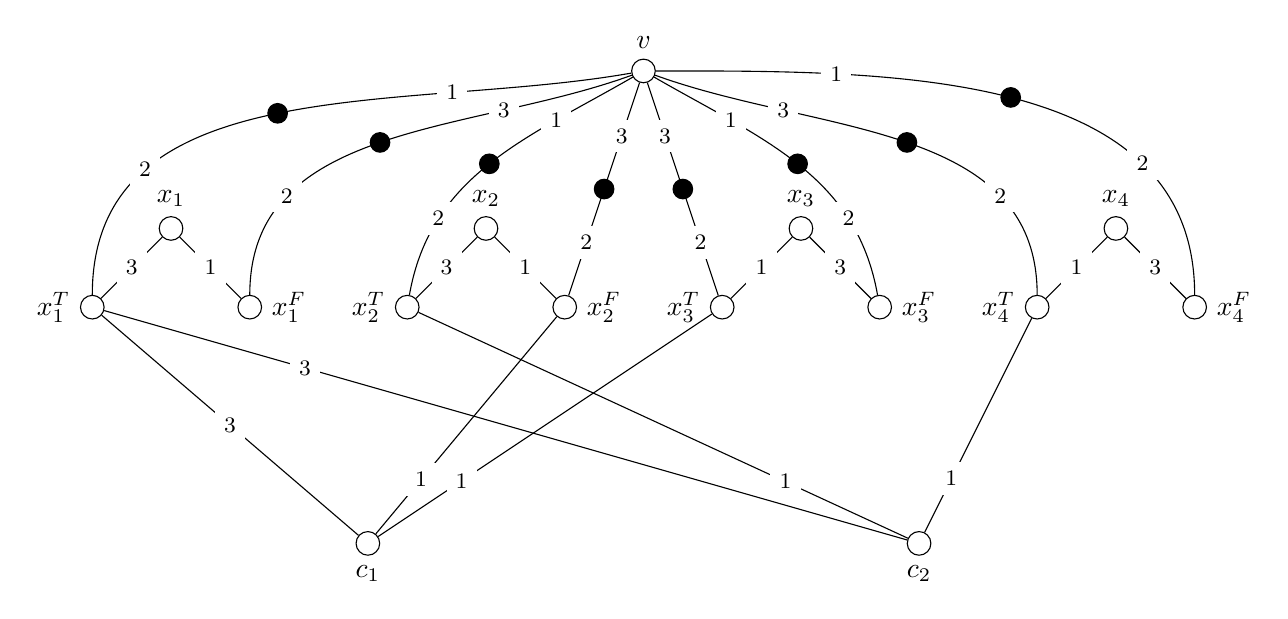
\begin{tikzpicture}%[xscale=2]

	%%Variable X1
	\node[vert,label=left:$x_1^T$] (x1t) at (1,0) {};
	\node[vert,label={[fill=white]right:$x_1^F$}] (x1f) at (3,0) {};
	\node[vert,label=above:$x_1$] (x1) at (2,1) {};
	
	%%Variable X2
	\node[vert,label={[fill=white]left:$x_2^T$}] (x2t) at (5,0) {};
	\node[vert,label={[fill=white]right:$x_2^F$}] (x2f) at (7,0) {};
	\node[vert,label={[fill=white]above:$x_2$}] (x2) at (6,1) {};
	
	%%Variable x3
	\node[vert,label={[fill=white]left:$x_3^T$}] (x3t) at (9,0) {};
	\node[vert,label={[fill=white]right:$x_3^F$}] (x3f) at (11,0) {};
	\node[vert,label={[fill=white]above:$x_3$}] (x3) at (10,1) {};
	
	%%Variable x4
	\node[vert,label={[fill=white]left:$x_4^T$}] (x4t) at (13,0) {};
	\node[vert,label=right:$x_4^F$] (x4f) at (15,0) {};
	\node[vert,label=above:$x_4$] (x4) at (14,1) {};
	
	%%vertices for clauses c1, c2 + vertex v
	\node[vert,label=above:$v$] (v) at (8,3) {};
	\node[vert,label=below:$c_1$] (c1) at (4.5,-3) {};
	\node[vert,label=below:$c_2$] (c2) at (11.5,-3) {};

    %%%%%% EDGES
    
	%%% edges between x1 gadget and v,c1,c2
    %x1 is TRUE
    %x1 to clause
    \draw (x1t) to node[timelabel] {$3$} (c1);
	\draw (x1t) to node[timelabel,pos=0.25] {$3$} (c2);
    %x1 gadget
    \draw (x1t) to [out=90,in=190] node[dummy] {} 
    node[timelabel,pos=0.25]{$2$} node[pos=0.75,timelabel]{$1$} (v);
	\draw (x1f) to [out=90,in=200] node[dummy] {}
    node[timelabel,pos=0.25]{$2$} node[pos=0.75,timelabel]{$3$} (v);
    \draw (x1t) to node[timelabel] {$3$} (x1) to node[timelabel] {$1$} (x1f);
	
	%%% edges between x2 gadget and v,c1,c2
    %x2 is TRUE
    %x2 to clause
	\draw (x2f) to node[timelabel,pos=0.75] {$1$} (c1);
	\draw (x2t) to node[timelabel,pos=0.75] {$1$} (c2);
    %x2 gadget
	\draw (x2t) to [out=80,in=210] node[dummy] {} 
    node[timelabel,pos=0.25]{$2$} node[pos=0.75,timelabel]{$1$} (v);
	\draw (x2f) to node[dummy] {} 
    node[timelabel,pos=0.25]{$2$} node[pos=0.75,timelabel]{$3$} (v);
    \draw (x2t) to node[timelabel] {$3$} (x2) to node[timelabel] {$1$} (x2f);

    %% edges between x3 gadget and v,c1
    %x3 is FALSE
    %x3 to clause
	\draw (x3t) to node[timelabel,pos=0.75] {$1$} (c1);
    %x3 gadget
	\draw (x3t) to node[dummy] {} 
    node[timelabel,pos=0.25]{$2$} node[pos=0.75,timelabel]{$3$} (v);
	\draw (x3f) to [out=100,in=330] node[dummy] {} 
    node[timelabel,pos=0.25]{$2$} node[pos=0.75,timelabel]{$1$} (v);
    \draw (x3t) to node[timelabel, pos=0.5] {$1$} (x3) to node[timelabel, pos=0.5] {$3$} (x3f);
	
    %%% edges between x4 gadget and v,c2
    %x4 is false
    %x4 to clause
	\draw (x4t) to node[timelabel,pos=0.75] {$1$} (c2);
    %x4 gadget
	\draw (x4t) to [out=90,in=340] node[dummy] {} 
    node[timelabel,pos=0.25]{$2$} node[pos=0.75,timelabel]{$3$} (v);
	\draw (x4f) to [out=90,in=360] node[dummy] {} 
    node[timelabel,pos=0.25]{$2$} node[pos=0.75,timelabel]{$1$} (v);
    \draw (x4t) to node[timelabel, pos=0.5] {$1$} (x4) to node[timelabel, pos=0.5] {$3$} (x4f);
	
\end{tikzpicture}
}
\caption{Illustration of the temporal graph $(G,\lambda)$ from the NP-hardness reduction, 
	where the NAE 3-SAT formula $\phi$ is of form $\phi = \text{NAE}(x_1, \overline{x}_2, x_3) \wedge \text{NAE}(x_1, x_2, x_4)$.
    Presented is the labeling of $G$ corresponding to the assignment $x_1=x_2=\textsc{true}$ and $x_3,x_4=\textsc{false}$.
}\label{fig:NP-example}
\end{figure}

\end{proof}
	
\clearpage

\section{Ideas}
\begin{itemize}
    \item Symmetric distance matrix $D$: polytime?
    \item Use $|D|_\infty$ (maximum value in $D$) + max degree $\Delta$ as parameter $\rightarrow$ should give FPT
    \item FPT with feedback edge number
    \item use as parameter $\max_{i,j} |D_{i,j}-D_{j,i}|$
    \item approximation (additive or multiplicative), maybe with graph as input
\end{itemize}

\problemdef{\kDeltaExactLong\ (\kDeltaExact)}
{An $n \times n$ matrix $D$ of positive integers.}
{Does there exist a graph $G=(V,E)$ with vertices $\{v_1,\ldots,v_{n}\}$ 
and a $\Delta$-periodic labeling $\lambda: E \rightarrow \{1,2,\ldots,\Delta\}^k$ such that, 
for every $i,j$, the duration of the fastest temporal path from $v_i$ to $v_j$ in the $\Delta$-periodic temporal graph $(G,\lambda,\Delta)$ is equal to $D_{i,j}$.}

\problemdef{\DeltaUpperBoundLong}
{An $n \times n$ matrix $D$ of positive integers and an integer $k\in \mathbb{N}$.}
{Does there exist a graph $G=(V,E)$ with vertices $\{v_1,\ldots,v_{n}\}$ with $n+k-1$ edges 
	and a $\Delta$-periodic labeling $\lambda: E \rightarrow \{1,2,\ldots,\Delta\}$ such that, 
	for every $i,j$, the duration of the fastest temporal path from $v_i$ to $v_j$ in the $\Delta$-periodic temporal graph $(G,\lambda,\Delta)$ is \emph{at most} $D_{i,j}$.}

\problemdef{\kDeltaLowerBoundLong}
{An $n \times n$ matrix $D$ of positive integers and an integer $k\in \mathbb{N}$.}
{Does there exist a graph $G=(V,E)$ on the vertices $\{v_1,\ldots,v_{n}\}$ with $n+k-1$ edges 
and a $\Delta$-periodic labeling $\lambda: E \rightarrow \{1,2,\ldots,\Delta\}$ such that, 
for every $i,j$, the duration of the fastest temporal path from $v_i$ to $v_j$ in the $\Delta$-periodic temporal graph $(G,\lambda,\Delta)$ is \emph{at least} $D_{i,j}$.}
\todo[inline]{NOT TEMPORALLY INTERESTING: the difficulty is to find a static graph with equal labels}

\todo[inline]{The matrix $D$ is m x m, and capturing the distances from an edge e to an edge f (zoom 14 Nov 22, GH).}
\todo[inline]{Check if the reduction works for the UPPER BOUNDED version (seems to work)}
\todo[inline]{how to extend the poly algorithms of cycles? Easy candidate: FES, FVS, series-parallel graphs, or tw=2 graphs}
\todo[inline]{FVS, $c$-factor approximation, hardness of approximation for $c<1.5$}

\clearpage
\section{Old (not useful?) results}
\begin{proof}[Proof idea for \cref{thm:paths-upperBound} -- old:]
	Let $P = (v_1, v_2, \dots, v_n)$ be a path on $n$ vertices.
	For the sake of simplicity we denote with $a_i$ label of edge $e_i =v_iv_{i+1}$, for all $i \in [n-1]$.
	By the definition, for any two vertices $v_i,v_j \in P$, we have the following inequality:
	\begin{equation*}
		(a_{i+1} - a_i)_\Delta + (a_{i+2} - a_{i+1})_\Delta + \cdots + (a_{j-1} - a_{j-2})_\Delta + 1
		\leq D_{i,j}.
	\end{equation*}
	For the sake of simplicity we refer to the inequality that a temporal path from $v_i$ to $v_j$ has to respect (\ie~the above inequality) 
	as $I_{i,j}$.
	Note that we can rewrite the inequality $I_{i,j}$ also without the modulo $\Delta$ part as:
	\begin{equation*}
		k_{i+1,i} \Delta + (a_{i+1} - a_i)+ k_{i+2,i+1} \Delta + (a_{i+2} - a_{i+1}) + \cdots + k_{j-1,j-2} \Delta + (a_{j-1} - a_{j-2})+ 1
		\leq D_{i,j},
	\end{equation*}
	where all $k_{i,i+1} \in \{0,1\}$.
	
	W.l.o.g. we can assume also that $a_i \neq a_{i+1}$ for all $i \in [n-1]$,
	this follows from the fact that the duration among two vertices $v_i, v_{i+2}$ on distance $2$ in $P$ equals to $\Delta + 1$ when the two consecutive labels are the same, but if the labels are not the same, the duration can be at most $\Delta$, which still satisfies the condition from before.
	Therefore, for any two consecutive labels $a_i$ and $a_{i+1}$ (\ie for any two vertices $v_i, v_{i+2}$ on distance $2$ in $P$), 
	it follows that 
	$k_{i, i+1} = 1 - k_{i+1,i}$, where $k_{i+1,i} \in \{0,1\}$, which makes also $k_{i,i+1} \in \{0,1\}$, as required.
	If we now sum up the two inequalities $I_{i,i+2}, I_{i+2,i}$ we get the following:
	\begin{equation*}
		(a_i-a_{i+1})_\Delta + (a_{i+1}-a_i)_\Delta +1 +1 = \Delta + 2.
	\end{equation*}
	It follows that for any two vertices $v_i, v_j$ in $P$, that are on distance $k$ apart, 
	we get that $d(i,j) + d(j,i) = (k-1) \Delta + 2$.
	
	To satisfy the inequalities $I_{1,n}$ and $I_{n,1}$ we have to correctly determine which of $k_{i+1,i}$ have value $1$, and consequently set $k_{i,i+1} = 0$,
	and vice versa.
	
	From the value $D_{1,n}$ (resp.~$D_{n,1}$) we can determine how many of $k_{i+1,i}$ (resp.$k_{i,i+1}$) can be non-zero. Suppose that there are $m$ non-zero ones (resp.~$n-m-1$).
	Then to determine which $m$ of the $k_{i,i+1}$ are non-zero we look at every two vertices $v_i, v_{i+2}$ at the distance $2$ in $P$ 
	and based on the inequalities $I_{i,i+2}, I_{i+2,i}$ determine if $k_{i+1,i}$ has a value $1$ or $0$,
	i.e.~if $e_{i+1}$ is bigger or smaller than $e_i$.
	We start determining the values $k_{i+1,i}$ from ``left to right'' (i.e~first we determine $k_{2,1}$, then $k_{3,2}$, \dots, and at last $k_{i-1,i-2}$).
	Now that the relations of every two consecutive labels of $P$ are determined, 
	we select the values for each label, such that the inequalities among them hold.
	\begin{claim}
		The above procedure produces a labeling of $P$ that satisfies durations from $D$.
	\end{claim}
\end{proof}


\bibliography{bibliography}	
\end{document}
